
This chapter compares five of the multivariate approximation
techniques that operate on inputs in $\mathbb{R}^d$ ($d$-tuples of
real numbers) and produce predicted responses in $\mathbb{R}$. Three
of the chosen techniques are regression based and the remaining two
are interpolants, providing reasonable coverage of the varied
mathematical strategies that can be employed to solve continuous
modeling problems.

%     Methodology     
%=====================
\section{I/O Data}

In order to evaluate the viability of multivariate models for
predicting system performance, this work presents a case study of a
four-dimensional dataset produced by executing the IOzone benchmark
from \citet{iozone} on a homogeneous cluster of computers. Multiple
I/O Zone data sets will be used throughout the work, however this
chapter relies on this specific four-dimensional dataset. All
experiments were performed on parallel shared-memory nodes common to
HPC systems. Each system had a lone guest Linux operating system
(Ubuntu 14.04 LTS//XEN 4.0) on a dedicated 2TB HDD on a 2 socket, 4
core (2 hyperthreads per core) Intel Xeon E5-2623 v3 (Haswell)
platform with 32 GB DDR4. The system performance data was collected by
executing IOzone 40 times for each of a select set of system
configurations. A single IOzone execution reports the max I/O
throughput seen for the selected test in kilobytes per second. The 40
executions for each system configuration are converted into the mean
and variance, both values in $\mathbb{R}$ capable of being modeled
individually by the multivariate approximation techniques presented in
Chapter \ref{ch:algs}. The summary of data used in the experiments for
this chapter can be seen in Table \ref{tab:data_type}.  Distributions
of raw throughput values being modeled can be seen in Figure
\ref{fig:raw_throughput}.

\begin{table}
  \centering
  \begin{tabular}{c|c}
    \hline
    \textbf{System Parameter} & \textbf{Values}\\
    \hline
    File Size & 64, 256, 1024\\
    Record Size & 32, 128, 512\\
    Thread Count & 1, 2, 4, 8, 16, 32, 64, 128, 256\\
    Frequency & \{12, 14, 15, 16, 18, 19, 20, 21, 23, 24, 25, 27, 28, 29, 30, 30.01\} $\times 10^5$\\
    \hline
    \textbf{Response Values} & \\
    \hline
    Throughput Mean & [$2.6 \times 10^5$, $5.9 \times 10^8$]\\
    Throughput Variance & [$5.9\times 10^{10} $, $4.7 \times 10^{16}$]\\
    \hline
  \end{tabular}
  \caption{A description of the system parameters being considered in
    the IOzone tests. Record size must not be greater than file size
    and hence there are only six valid combinations of the two. In
    total there are $6 \times 9 \times 16 = 864$ unique system
    configurations.}
  \label{tab:data_type}
\end{table}

\begin{figure}
  \centering
  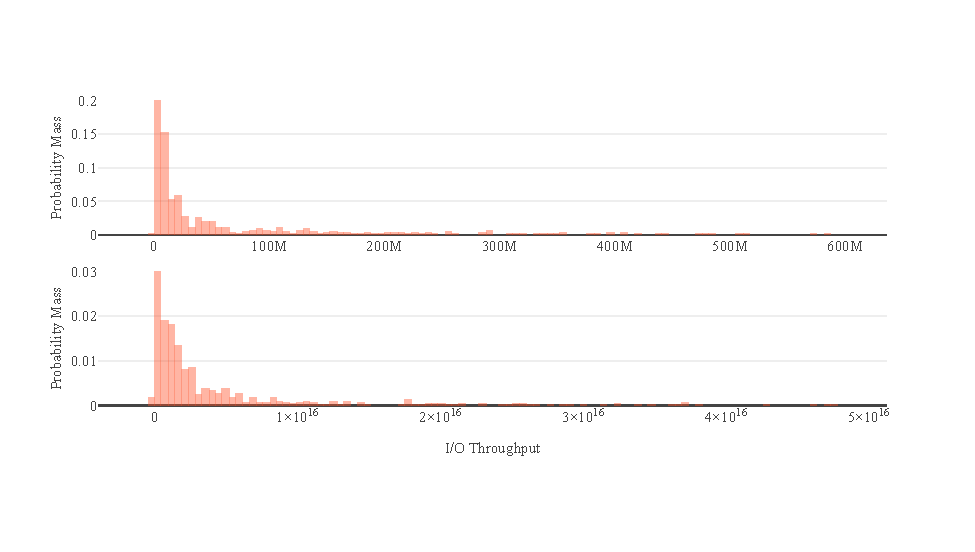
\includegraphics[width=\textwidth,trim={0 .5in 0 .4in}]{Figures/HPC/Raw_Throughput.pdf}
  \caption{Histograms of 100-bin reductions of the PMF of I/O
    throughput mean (top) and I/O throughput variance (bottom). In the
    mean plot, the first 1\% bin (truncated in plot) has a probability
    mass of .45. In the variance plot, the second 1\% bin has a
    probability mass of .58. It can be seen that the distributions of
    throughputs are primarily of lower magnitude with occasional
    extreme outliers.}
  \label{fig:raw_throughput}
\end{figure}

\subsection{Dimensional Analysis}

This analysis utilizes an extension to standard $k$-fold cross
validation that allows for a more thorough investigation of the
expected model performance in a variety of real-world
situations. Alongside randomized splits, two extra components are
considered: the amount of training data provided, and the dimension of
the input data. It is important to consider that algorithms that
perform well with less training input also require less
experimentation. Although, the amount of training data required may
change as a function of the dimension of the input and this needs to
be studied as well. The framework used here will be referred to as a
multidimensional analysis (MDA) of the IOzone data.

\subsubsection{Multidimensional Analysis}

This procedure combines random selection of training and testing
splits with changes in the input dimension and the ratio of training
size to testing size. Given an input data matrix with $n$ rows
(points) and $d$ columns (components), MDA proceeds as follows:
\begin{enumerate}
\item For all $k = 1$, $\ldots$, $d$ and for all nonempty subsets $F
  \subset \{1, 2, \ldots, d\}$, reduce the input data to points $(z,
  f_F(z))$ with $z \in \mathbb{R}^k$ and $f_F(z) = E\bigl[ \bigl\{
    f\bigl(x^{(i)}\bigr) \bigm| \bigl(x^{(i)}_F = z\bigr) \bigr\}
    \bigr]$, where $E[\cdot]$ denotes the mean and $x^{(i)}_F$ is the
  subvector of $x^{(i)}$ indexed by $F$.
\item For all $r$ in $\{5, 10, \ldots, 95\}$, generate $N$ random
  splits $(train, test)$ of the reduced data with $r$ percentage for
  training and $100 - r$ percentage for testing.
\item When generating each of $N$ random $(train, test)$ splits,
  ensure that all points from $test$ are in the convex hull of points
  in $train$ (to prevent extrapolation); also ensure that the points
  in $train$ are well spaced.
\end{enumerate}

In order to ensure that the testing points are in the convex hull of
the training points, the convex hull vertices of each set of (reduced
dimension) points are forcibly placed in the training set. In order to
ensure that training points are well spaced, a statistical method for
picking points from \citet{amos2014algorithm} is used:
\begin{enumerate}
\item Generate a sequence of all pairs of points
  $\bigl(z^{(i_1)},z^{(j_1)}\bigr), \bigl(z^{(i_2)},z^{(j_2)}\bigr),
  \ldots$ sorted by ascending pairwise Euclidean distance between
  points, so that $\bigl|\bigl|z^{(i_k)}-z^{(j_k)}\bigr|\bigr|_2 \leq
  \bigl|\bigl|z^{(i_{k+1})}-z^{(j_{k+1})}\bigr|\bigr|_2$.
\item Sequentially remove points from candidacy until only $|train|$
  remain by randomly selecting one point from the pair
  $\bigl(z^{(i_m)}, z^{(j_m)}\bigr)$ for $m = 1,\ldots$ if both
  $z^{(i_m)}$ and $z^{(j_m)}$ are still candidates for removal.
\end{enumerate}

Given the large number of constraints, level of reduction, and use of
randomness in the MDA procedure, occasionally $N$ unique
training/testing splits may not be created or may not exist. In these
cases, if there are fewer than $N$ possible splits, then
deterministically generated splits are used. Otherwise after $3N$
attempts, only the unique splits are kept for analysis. The MDA
procedure has been implemented in Python\#3 while most regression and
interpolation methods are Fortran wrapped with Python. All randomness
has been seeded for repeatability.

For any index subset $F$ (of size $k$) and selected value of $r$, MDA
will generate up to $N$ multivariate models $f_F(z)$ and predictions
$\hat{f}_F\big(z^{(i)}\big)$ for a point $z^{(i)} \in \mathbb{R}^k$.
There may be fewer than $N$ predictions made for any given
point. Extreme points of the convex hull for the selected index subset
will always be used for training, never for testing. Points that do
not have any close neighbors will often be used for training in order
to ensure well-spacing. Finally, as mentioned before, some index
subsets do not readily generate $N$ unique training and testing
splits. The summary results presented in this work use the median of
the ($N$ or fewer) values $\hat{f}_F(z)$ at each point as the model
estimate for error analysis.


\section{Na\"{\i}ve Variability Modeling Results}

A na\"{\i}ve multivariate prediction technique such as nearest
neighbor could experience relative errors in the range $\displaystyle
[0, \big(\max_x f(x) - \min_x f(x)\big) / \min_x f(x) ]$ when modeling
a nonnegative function $f(x)$ from data. The IOzone mean data response
values span three orders of magnitude (as can be seen in Table
\ref{tab:data_type}) while variance data response values span six
orders of magnitude. It is expected therefore, that all studied
multivariate models perform better than a na\"{\i}ve approach,
achieving relative errors strictly less than $10^3$ for throughput
mean and $10^6$ for throughput variance. Ideally, models will yield
relative errors significantly smaller than 1. The time required to
compute thousands of models involved in processing the IOzone data
through MDA was approximately five hours on a CentOS workstation with
an Intel i7-3770 CPU at 3.40GHz. In four dimensions for example, each
of the models could be constructed and evaluated over hundreds of
points in less than a few seconds.


\subsection{I/O Throughput Mean}

Almost all multivariate models analyzed make predictions with a
relative error less than 1 for most system configurations when
predicting the mean I/O throughput of a system given varying amounts
of training data. The overall best of the multivariate models,
Delaunay, consistently makes predictions with relative error less than
$.05$ (5\% error). In Figure \ref{fig:mean_tt_ratio} it can also be
seen that the Delaunay model consistently makes good predictions even
with as low as 5\% training data (43 of the 864 system configurations)
regardless of the dimension of the data.

\begin{figure}
  \centering
  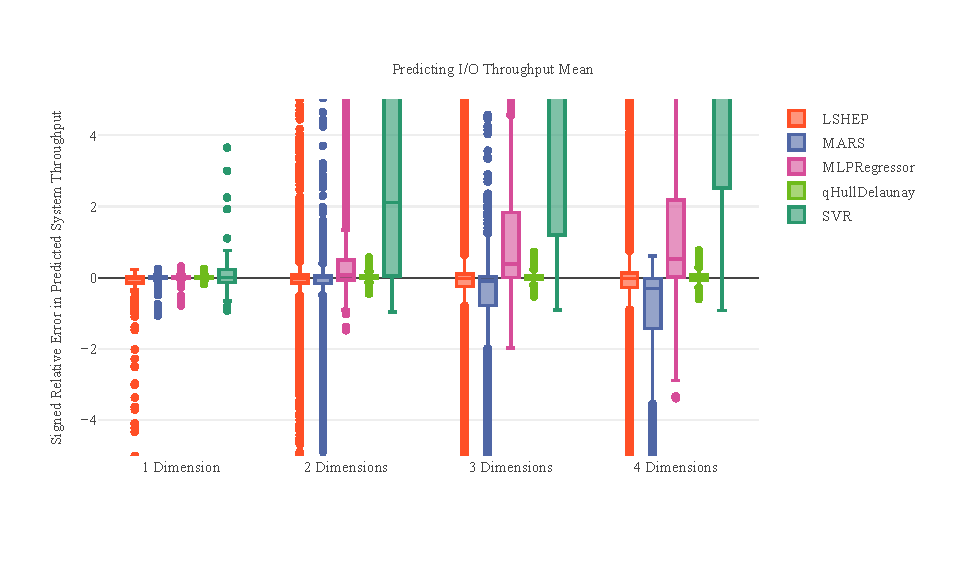
\includegraphics[width=\textwidth,trim={0 .5in 0 .3in}]{Figures/HPC/Mean_Dim.pdf}
  \caption{These box plots show the prediction error of mean with
    increasing dimension. The top box whisker for SVR is 40, 80, 90
    for dimensions 2, 3, and 4, respectively. Notice that each model
    consistently experiences greater magnitude error with increasing
    dimension. Results for all training percentages are aggregated.}
  \label{fig:mean_dim}
\end{figure}

\begin{figure}
  \centering
  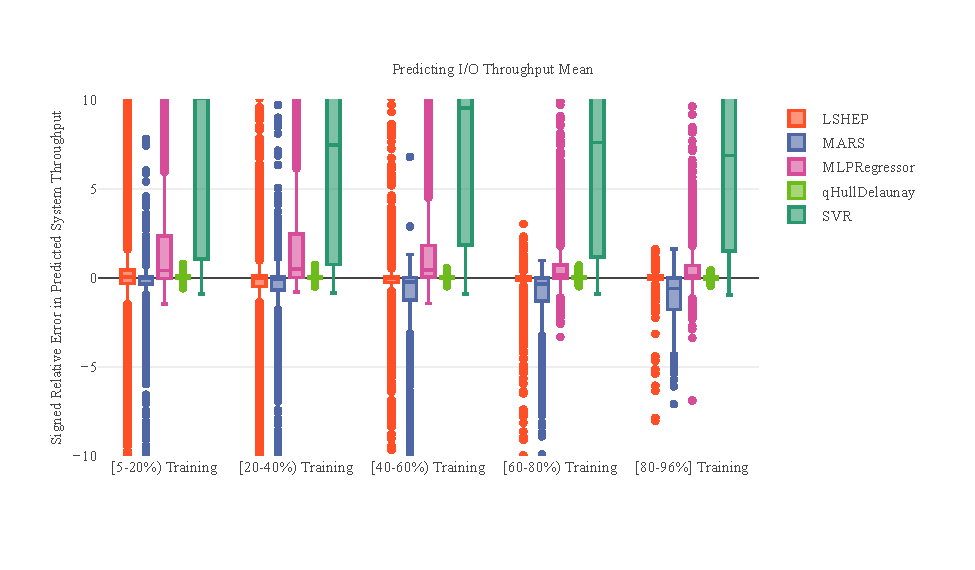
\includegraphics[width=\textwidth,trim={0 .5in 0 .3in}]{Figures/HPC/Mean_TT_Ratio.pdf}
  \caption{These box plots show the prediction error of mean with
    increasing amounts of training data provided to the models. Notice
    that MARS is the only model whose primary spread of performance
    increases with more training data. Recall that the response values
    being predicted span three orders of magnitude and hence relative
    errors should certainly remain within that range. For SVR the top
    box whisker goes from around 100 to 50 from left to right and is
    truncated in order to maintain focus on better models. Results for
    all dimensions are aggregated. Max training percentage is 96\% due
    to rounding training set size.}
  \label{fig:mean_tt_ratio}
\end{figure}

\begin{figure}
  \centering
  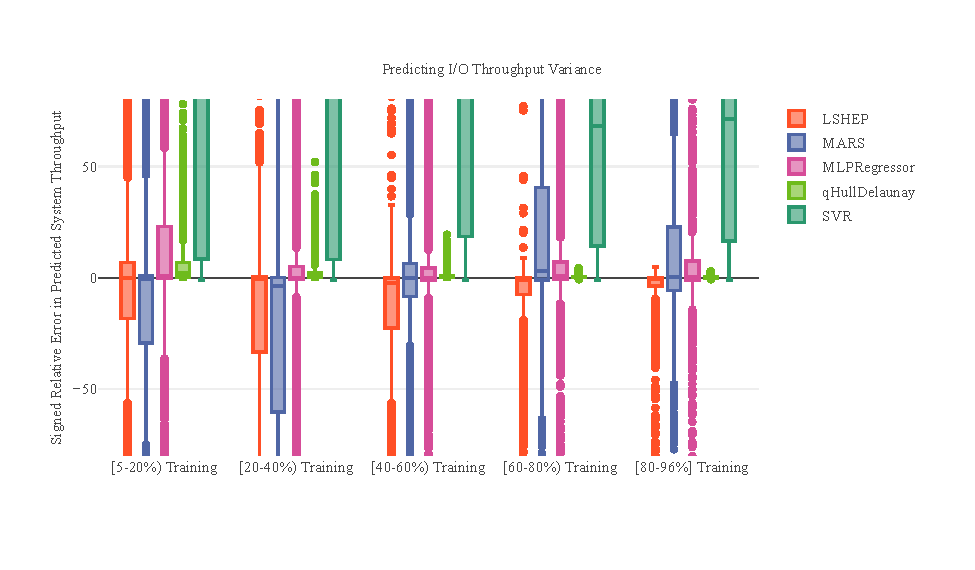
\includegraphics[width=\textwidth,trim={0 .5in 0 .3in}]{Figures/HPC/Var_TT_Ratio.pdf}
  \caption{These box plots show the prediction error of variance with
    increasing amounts of training data provided to the models. The
    response values being predicted span six orders of magnitude. For
    SVR the top box whisker goes from around 6000 to 400 (decreasing
    by factors of 2) from left to right and is truncated in order to
    maintain focus on better models. Results for all dimensions are
    aggregated. Max training percentage is 96\% due to rounding
    training set size.}
  \label{fig:var_tt_ratio}
\end{figure}
 

\subsection{I/O Throughput Variance}

The prediction results for variance resemble those for
predicting mean. Delaunay remains the best overall predictor
(aggregated across training percentages and dimensions) with median
relative error of .47 and LSHEP closely competes with Delaunay having
a median signed relative error of -.92. Outliers in prediction error
are much larger for all models. Delaunay produces relative errors as
large as 78 and other models achieve relative errors around
$10^3$. The relative errors for many models scaled proportional to the
increased orders of magnitude spanned by the variance response
compared with mean response. As can be seen in Figure
\ref{fig:var_tt_ratio}, all models are more sensitive to the amount of
training data provided than their counterparts for predicting mean.

\subsection{Increasing Dimension and Decreasing Training Data}

As can be seen in Figure \ref{fig:mean_dim}, all of the models suffer
increasing error rates in higher dimension. This is expected, because
the number of possible interactions to model grows
exponentially. However, LSHEP and Delaunay maintain the slowest
increase in relative error. The increase in error seen for Delaunay
suggests that it is capable of making predictions with a range of
relative errors that grows approximately linearly with increasing
dimension input. This trend suggests that Delaunay would remain a
viable technique for accurately modeling systems with 10's of
parameters given only small amounts of training data. All models, with
the exception of MARS, produce smaller errors given more training
data. Increasing the amount of training data most notably reduces the
number of prediction error outliers.

%     Discussion     
%====================
\section{Discussion of Na\"{\i}ve Approximations}

The results presented above demonstrate that a straightforward
application of multivariate modeling techniques can be used to
effectively predict HPC system performance. Some modeling effort on
the part of a systems engineer combined with a significant amount of
experimentation (days of CPU time for the IOzone data used here) can
yield a model capable of accurately tuning an HPC system to the
desired performance specification, although qualitatively correct
predictions can be achieved with much less (10\%, say) effort.

\subsection{Modeling the System}

The modeling techniques generated estimates of drastically different
quality when predicting I/O throughput mean and variance. A few
observations: SVR has the largest range of errors for all selections
of dimension and amounts of training data; MARS and LSHEP produce
similar magnitude errors while the former consistently underestimates
and the latter consistently overestimates; Delaunay has considerably
fewer outliers than all other methods. SVR likely produces the poorest
quality predictions because the underlying parametric representation
is global and oversimplified (a single polynomial), making it unable
to capture the complex local behaviors of system I/O. It is still
unclear, however, what causes the behaviors of LSHEP, MARS, and
Delaunay. An exploration of this topic is left to future work.

The Delaunay method appears to be the best predictor in the present
IOzone case study. Particularly a piecewise linear interpolant like
Delaunay appears well-suited for prediction when relatively small
amounts of data are available to mode la function. It is important to
note that the Delaunay computational complexity in the dimension of
the input is worse than other techniques.

Finally, the ability of the models to predict variance was
significantly worse than for the I/O mean. The larger scale in
variance responses alone do not account for the increase in relative
errors witnessed. This suggests that system variability has a greater
underlying functional complexity than the system mean and that latent
factors are reducing prediction performance.

\subsection{Extending the Analysis}

System I/O throughput mean and variance are simple and useful system
characteristics to model. The process presented in this chapter is
equally applicable to predicting other useful performance
characteristics of HPC systems such as: computational throughput,
power consumption, processor idle time, context switches, RAM usage,
or any other ordinal performance metric. For each of these there is
the potential to model system variability as well. This chapter uses
variance as a measure of variability, but the techniques are applied
to more precise measures of variability (the entire distribution
itself) in Chapter \ref{ch:strong}.

\vspace{-10pt}
\section{Takeaway From Na\"{\i}ve Approximation}
\label{sec:conclusion}

Multivariate models of HPC system performance can effectively predict
I/O throughput mean and variance. These multivariate techniques
significantly expand the scope and portability of statistical models
for predicting computer system performance over previous work. In the
IOzone case study presented, the Delaunay method produces the best
overall results making predictions for 821 system configurations with
less than 5\% error when trained on only 43 configurations. Analysis
also suggests that the error in the Delaunay method will remain
acceptable as the number of system parameters being modeled
increases. These multivariate techniques should be applied to HPC
systems with more than four tunable parameters in order to identify
optimal system configurations that may not be discoverable via
previous methods nor by manual performance tuning, which will be
explored in later chapters.
